\chapter{実験結果}
本章では,前章で説明したトレーディングアルゴリズムを使って上位東証上位100社のうち2013年からのデータがある95株の
平均利益,平均勝率,最適化した平均$tp$,$ls$,平均トレード数を評価する.
\section{実験環境}
本研究における実験環境を表\ref{env}と\ref{lib}に表す.

\begin{table}[hbtp]
 \centering
 \caption{実験環境}
  \label{env}
 \begin{tabular}{|l||l|}
   \hline
   OS & Ubuntu 22.04.3 LTS\\
   \hline
   CPU & Intel Core i9-9900K\\
   \hline
   メモリ & 128GB \\
   \hline
   言語 & Python 3.10.12 \\
   \hline
  \end{tabular}
\end{table}

\begin{table}[hbtp]
  \centering
  \caption{ライブラリのバージョン}
   \label{lib}
  \begin{tabular}{|l||l|}
    \hline
    \textbf{ライブラリ} & \textbf{バージョン}\\
    \hline
    Backtesting & 0.3.3\\
    \hline
    ta-lib-bin & 0.4.26\\
    \hline
    numpy & 1.26.0 \\
    \hline
    pandas & 1.5.3 \\
    \hline
    matplotlib & 3.8.0 \\
    \hline
   \end{tabular}
 \end{table}
\newpage
\section{上位95社の株価データ}

検証で使った株価データのコードを表\ref{data}に表す.上位東証上位100社のうち2013年からのデータがある95株を使用する.

\begin{table}[htbp]
  \centering
  \caption{株コード}
  \label{data}
  \begin{tabular}{|l|l|l|l|l|}
  \hline
  \multicolumn{5}{|c|}{\textbf{株コード}} \\
  \hline
  
  1605 & 1925 & 1928 & 2502 & 2503 \\
  \hline
  2802 & 2914 & 3382 & 4063 & 4307 \\
  \hline
  4452 & 4502 & 4503 & 4507 & 4519 \\
  \hline
  4523 & 4543 & 4568 & 4578 & 4612 \\
  \hline
  4661 & 4684 & 4689 & 4901 & 4911 \\
  \hline
  5108 & 5401 & 6146 & 6201 & 6273 \\
  \hline
  6301 & 6326 & 6367 & 6501 & 6502 \\
  \hline
  6503 & 6594 & 6701 & 6702 & 6723 \\
  \hline
  6752 & 6758 & 6762 & 6857 & 6861 \\
  \hline
  6902 & 6920 & 6954 & 6971 & 6981 \\
  \hline
  7011 & 7201 & 7203 & 7267 & 7269 \\
  \hline
  7270 & 7532 & 7733 & 7741 & 7751 \\
  \hline
  7832 & 7974 & 8001 & 8002 & 8015 \\
  \hline
  8031 & 8035 & 8053 & 8058 & 8113 \\
  \hline
  8267 & 8306 & 8308 & 8309 & 8316 \\
  \hline
  8411 & 8591 & 8604 & 8630 & 8725 \\
  \hline
  8750 & 8766 & 8801 & 8802 & 9020 \\
  \hline
  9022 & 9101 & 9432 & 9433 & 9503 \\
  \hline
  9613 & 9735 & 9843 & 9983 & 9984 \\
  \hline
  \end{tabular}
\end{table}

これらの株価データの入手方法を以下に示す.
\begin{enumerate}
 \item まずはじめにhttps://finance.yahoo.comに行く.
 \item 次に検索バーに株コードを入れると候補欄が出てくるのでそこで選択する.
 \item 出てきたページのHistorical Dataを選択する.
 \item Time Periodの項目があるので選択して株価データの使う期間を選択する.本論文では2013年1月1日から2022年12月31日のデータを使う.
 \item Applyボタンがあるので押してその下にあるDownloadボタンを押せば,株価データのcsvファイルを取得することができる.
\end{enumerate}

\section{トレーディングアルゴリズムの検証}
第3章で説明した$tp$,$sl$を最適化してそれぞれのアルゴリズムを実行し,結果を以下の表\ref{strategy_comparison}に表す.$tp$,$sl$はそれぞれ101~110%,-99~-90%で最適化する.
図\ref{fig:res1}は,表\ref{strategy_comparison}の平均利益,平均取引数,平均勝率をグラフ化したもので,図\ref{fig:res2}は,表\ref{strategy_comparison}の平均TP,平均SLをグラフ化したものである.

また,図\ref{fig:macdonysai}から図\ref{fig:bbandfmmacdsai}までのグラフは,アルゴリズム(B1)から(B13)によって得られた95社の株の利益である.
\begin{table}[htbp]
  \small
  \centering
  \caption{各戦略の比較}
  \label{strategy_comparison}
  \begin{tabular}{|l||l|l|l|l|l|}
    \hline
    
  \textbf{戦略} & \textbf{平均利益} & \textbf{平均TP} & \textbf{平均SL} & \textbf{平均勝率\%} & \textbf{平均取引数} \\
  \hline

  (B1) & 212.02144 & 107.95789 & 93.48421 & 53.80\% & 67.32 \\\hline
  (B2) & 95.86136 & 107.47368 & 93.34737 & 56.36\% & 35.80 \\\hline
  (B3) & 80.29327 & 107.63158 & 93.29474 & 56.22\% & 34.51 \\\hline
  (B4) & 63.71441 & 107.52632 & 93.46316 & 57.08\% & 24.82 \\\hline
  (B5) & 122.89338 & 107.37895 & 93.35789 & 56.44\% & 45.95 \\\hline
  (B6) & 125.71012 & 107.68421 & 93.00000 & 58.99\% & 40.18 \\\hline
  (B7) & 57.27753 & 106.90526 & 92.76842 & 64.45\% & 19.48 \\\hline
  (B8) & 51.61579 & 106.50526 & 92.62105 & 67.32\% & 19.21 \\\hline
  (B9) & 39.39328 & 106.83158 & 93.27368 & 66.21\% & 12.36 \\\hline
  (B10) & 69.63080 & 106.66316 & 92.47368 & 64.45\% & 26.14 \\\hline
  (B11) & 305.81290 & 107.41053 & 93.57895 & 53.82\% & 98.56 \\\hline
  (B12) & 123.13827 & 107.14737 & 93.65263 & 56.25\% & 50.98 \\\hline
  (B13) & 238.55610 & 107.80000 & 93.57895 & 53.21\% & 78.83 \\\hline
 
  \end{tabular}
\end{table}

\begin{figure}[H]
  \centering
  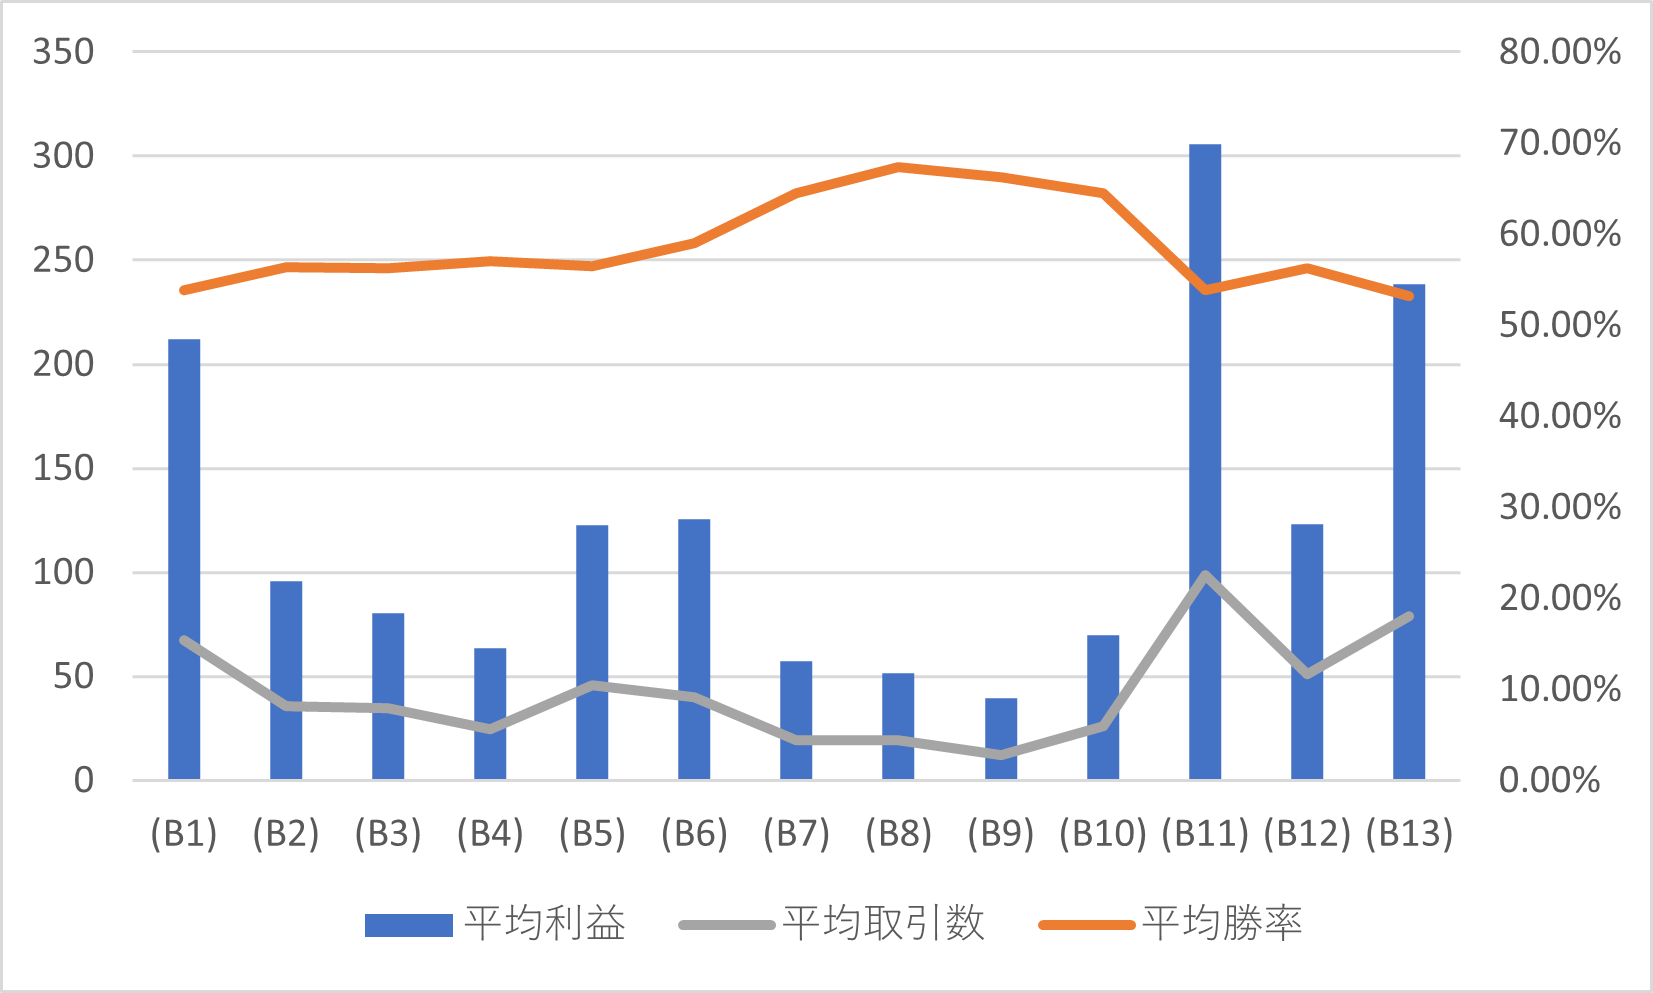
\includegraphics[width=110mm]{fig/res_1.png}
  \caption{平均利益,平均取引数,平均勝率のグラフ}
  \label{fig:res1}
 \end{figure}

 \begin{figure}[H]
  \centering
  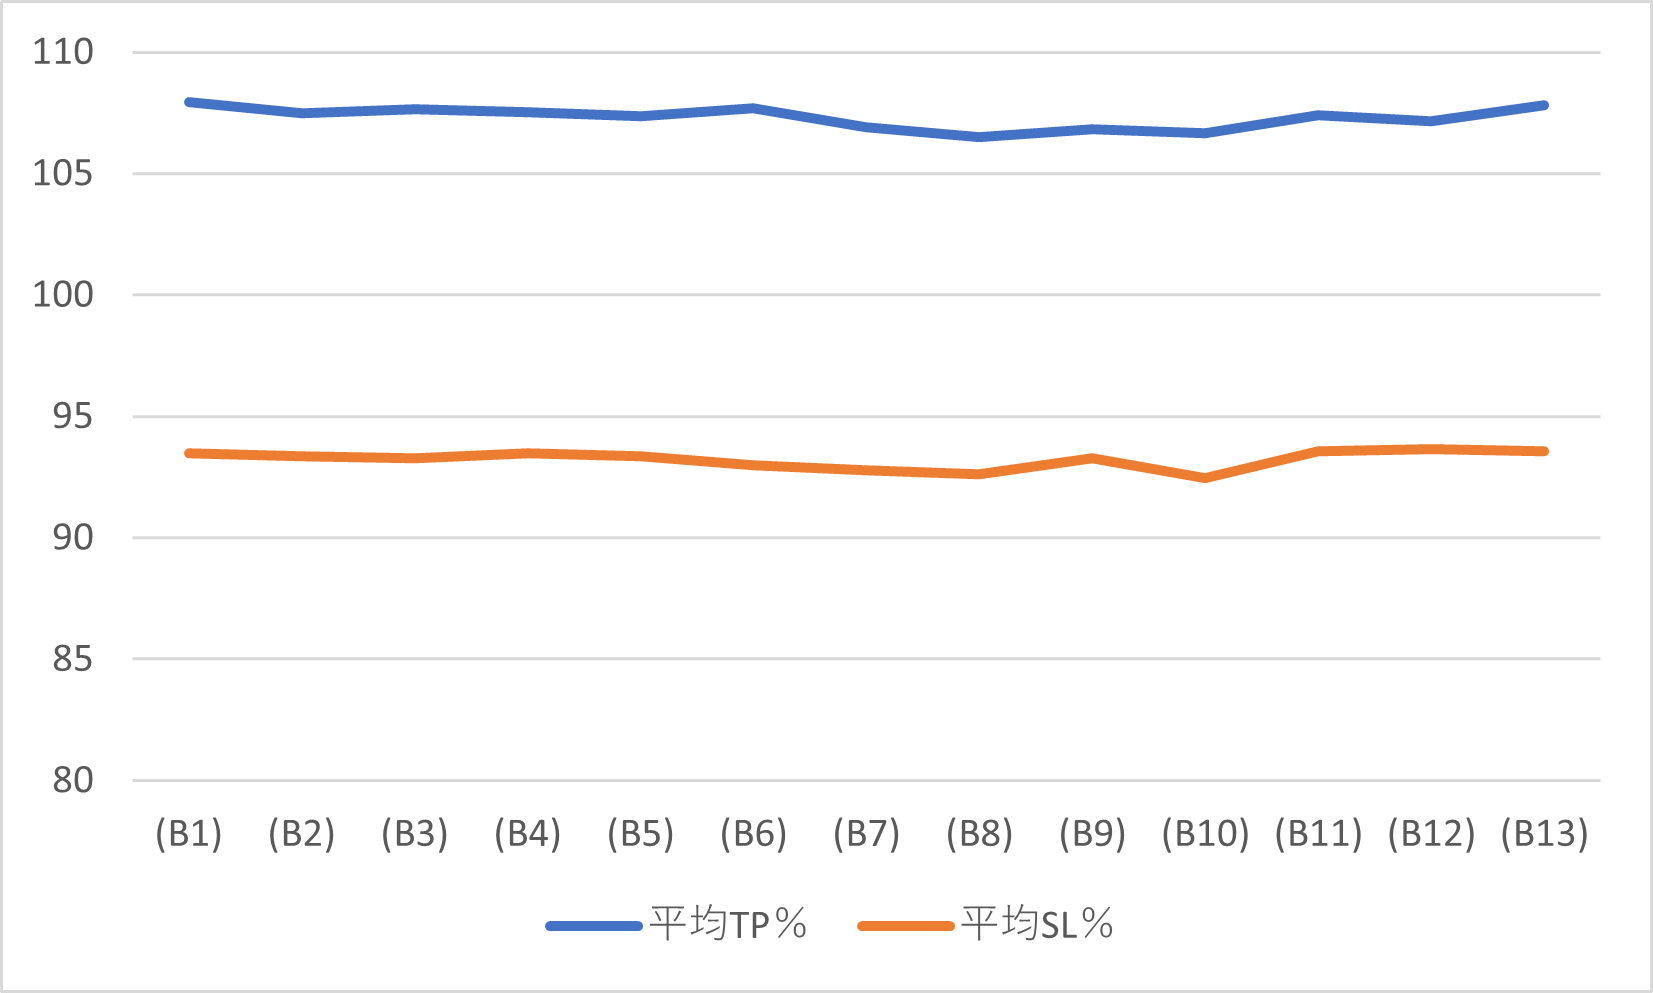
\includegraphics[width=110mm]{fig/res_2.png}
  \caption{平均SL,平均TPのグラフ}
  \label{fig:res2}
 \end{figure}

  \begin{figure}[H]
  \centering
  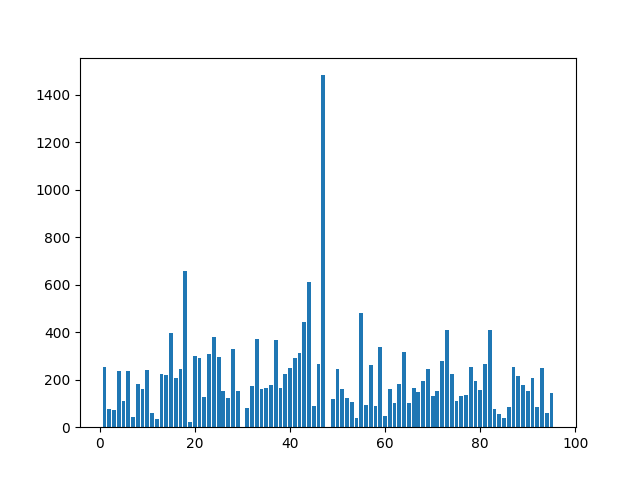
\includegraphics[width=110mm]{fig/macdonly_saiteki.png}
  \caption{アルゴリズムによる利益(B1)}
  \label{fig:macdonysai}
 \end{figure}

 \begin{figure}[H]
  \centering
  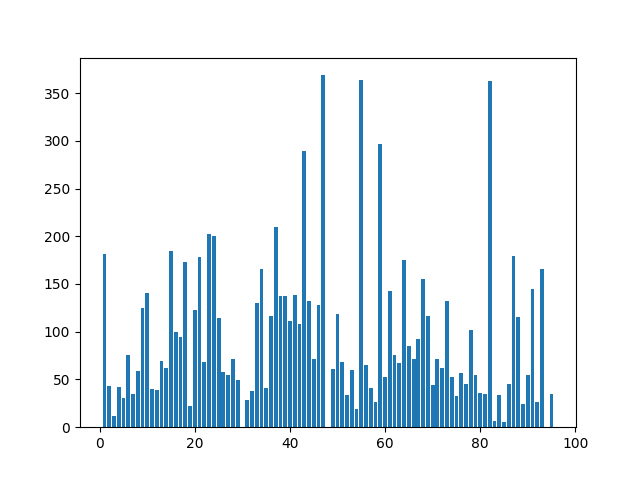
\includegraphics[width=110mm]{fig/macd_fma_saiteki.png}
  \caption{アルゴリズムによる利益(B2)}
  \label{fig:macdfmasai}
 \end{figure}

 \begin{figure}[H]
  \centering
  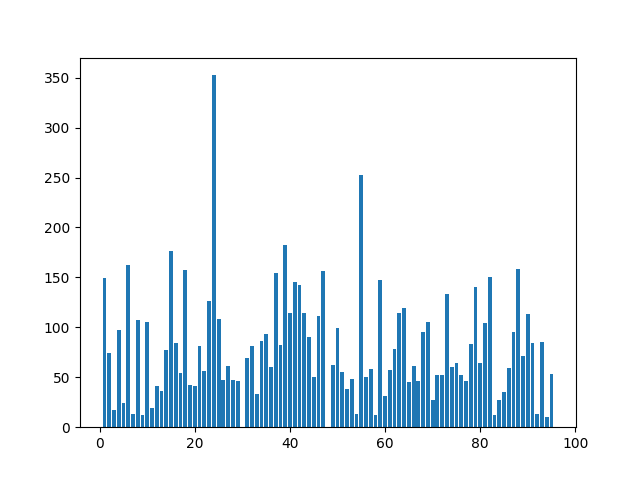
\includegraphics[width=110mm]{fig/macd_nikkei_saiteki.png}
  \caption{アルゴリズムによる利益(B3)}
  \label{fig:macdnikkeisai}
 \end{figure}

 \begin{figure}[H]
  \centering
  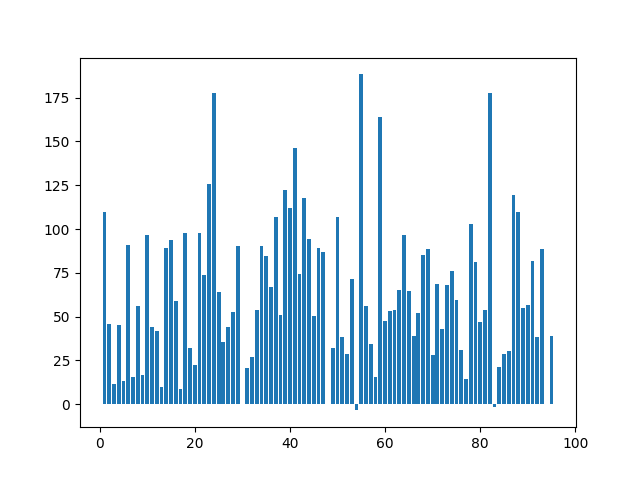
\includegraphics[width=110mm]{fig/macd_nikkeiandfma_saiteki.png}
  \caption{アルゴリズムによる利益(B4)}
  \label{fig:b4sai}
 \end{figure}

 \begin{figure}[H]
  \centering
  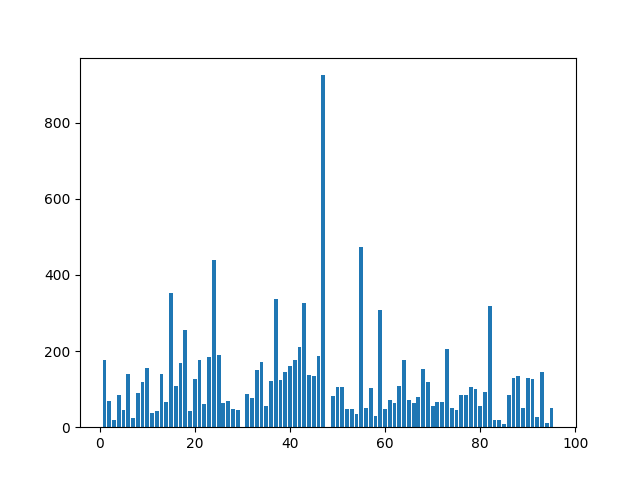
\includegraphics[width=110mm]{fig/macd_nikkeiorfma_saiteki.png}
  \caption{アルゴリズムによる利益(B5)}
  \label{fig:macdfmanksai}
 \end{figure}

 \begin{figure}[H]
  \centering
  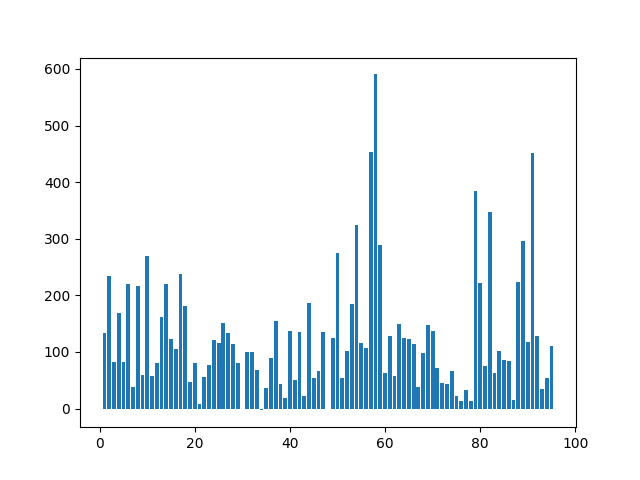
\includegraphics[width=110mm]{fig/bbonly_saiteki.png}
  \caption{アルゴリズムによる利益(B6)}
  \label{fig:bbsai}
 \end{figure}

 \begin{figure}[H]
  \centering
  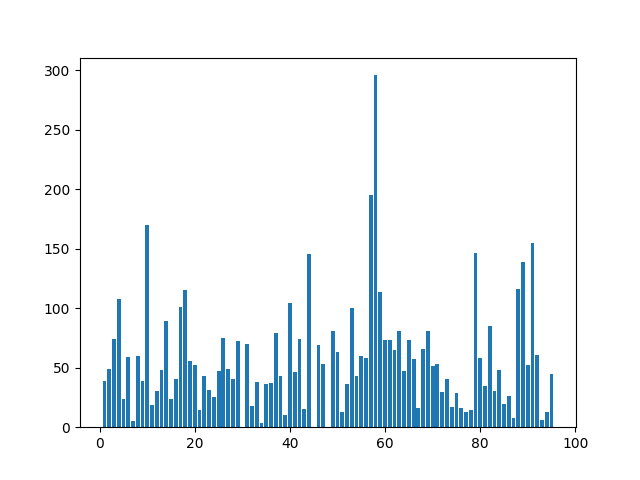
\includegraphics[width=110mm]{fig/bb_fma_saiteki.png}
  \caption{アルゴリズムによる利益(B7)}
  \label{fig:bbfmasai}
 \end{figure}

 \begin{figure}[H]
  \centering
  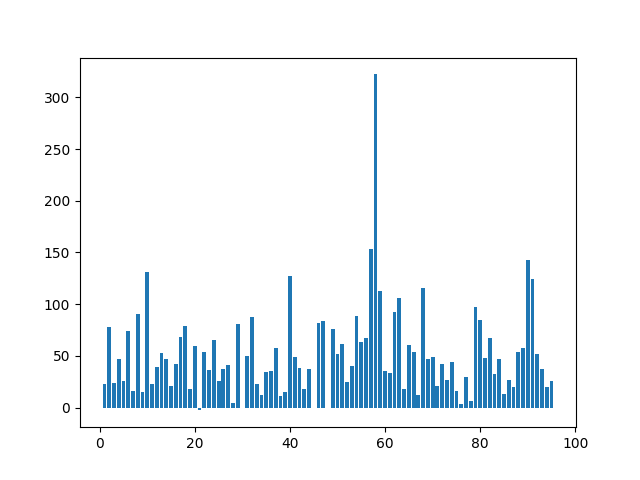
\includegraphics[width=110mm]{fig/bb_nikkei_saiteki.png}
  \caption{アルゴリズムによる利益(B8)}
  \label{fig:bbnikkeisai}
 \end{figure} 

 \begin{figure}[H]
  \centering
  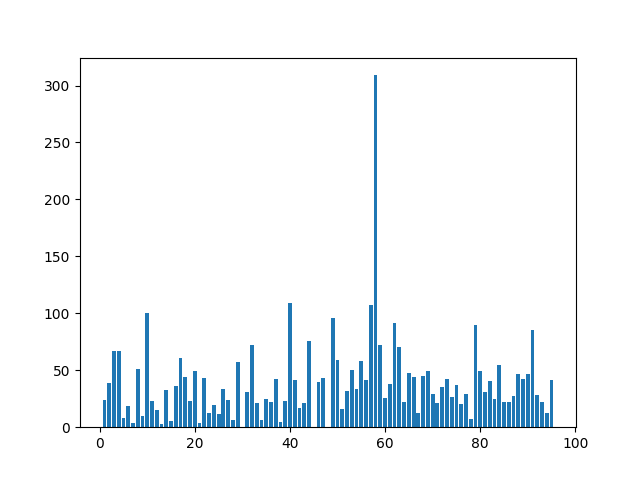
\includegraphics[width=110mm]{fig/bb_nikkeiandfma_saiteki.png}
  \caption{アルゴリズムによる利益(B9)}
  \label{fig:b9sai}
 \end{figure}

 \begin{figure}[H]
  \centering
  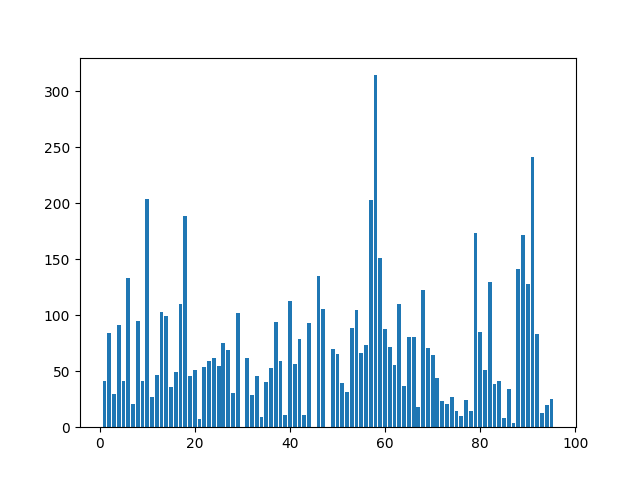
\includegraphics[width=110mm]{fig/bb_nikkeiorfma_saiteki.png}
  \caption{アルゴリズムによる利益(B10)}
  \label{fig:b10sai}
 \end{figure}

 \begin{figure}[H]
  \centering
  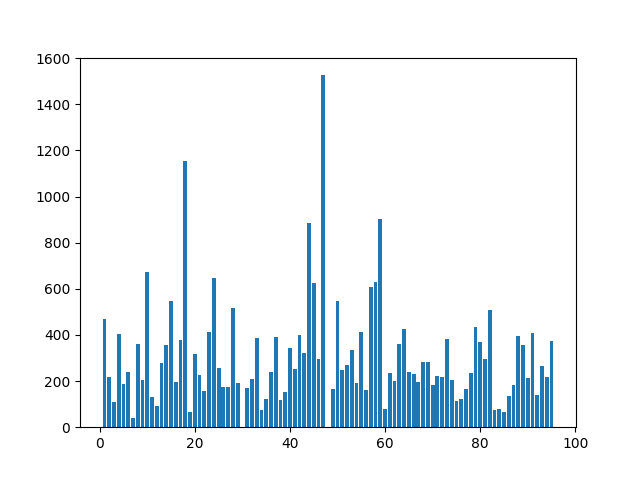
\includegraphics[width=110mm]{fig/bbmacdon_saiteki.png}
  \caption{アルゴリズムによる利益(B11)}
  \label{fig:bbmacdonsai}
 \end{figure}

 \begin{figure}[H]
  \centering
  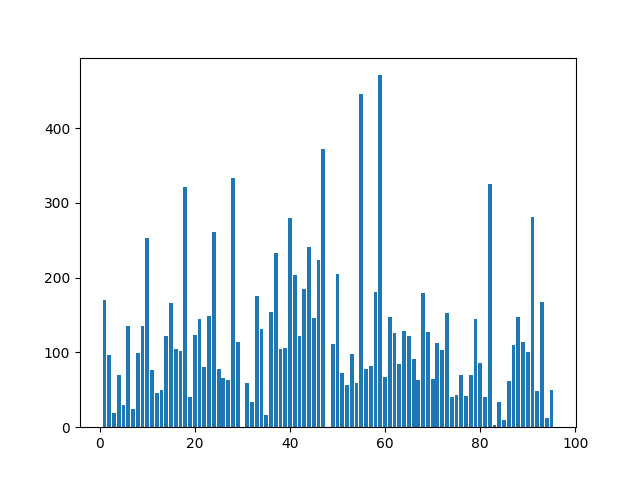
\includegraphics[width=110mm]{fig/bbmacdandfm_saiteki.png}
  \caption{アルゴリズムによる利益(B12)}
  \label{fig:bbmacdandfmsai}
 \end{figure}

 \begin{figure}[H]
  \centering
  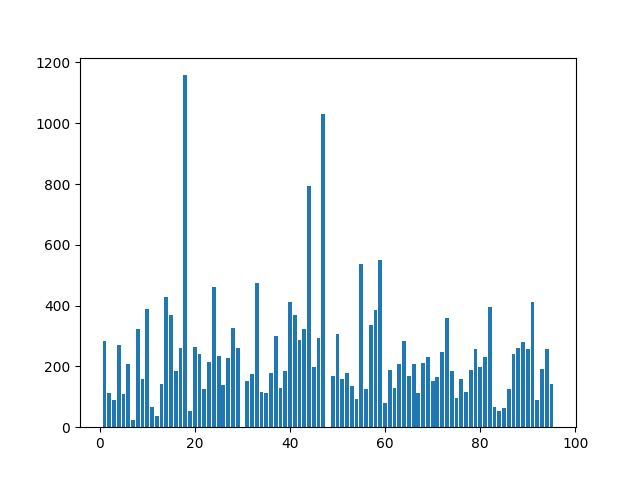
\includegraphics[width=110mm]{fig/bbandfmmacd_saiteki.png}
  \caption{アルゴリズムによる利益(B13)}
  \label{fig:bbandfmmacdsai}
 \end{figure}

\section{実験結果と考察}

表\ref{strategy_comparison}より,利確に適している値は約107%で,損切りに適している値は約93%.
勝率は高くて67%,低くても53%であることがわかる.
また,利益が一番高いのは(B11)であることがわかる.これは
既存のよく使われている2つ指標を組み合わせているためだと考えられる.
BBとMACDそれぞれ同じ条件の場合だとMACDの利益が高くBBの勝率が高い.
(B9)の場合はすべてが同時になるという条件が厳しいため,利益と取引が一番低いが勝率が高くなりやすいことがわかる.

利益だけを追い求めるならばMACD主体のトレーディングアルゴリズムか(B11)を選択すればいいが,リスクが少ない方法を選びのならばBB主体のトレーディングアルゴリズム選択すればよいことがわかる.
\newpage